\documentclass[12pt]{extarticle}
\usepackage{listings}
\usepackage{amsmath,amssymb}
\usepackage{xcolor}
\usepackage[]{caption}

\definecolor{codegreen}{rgb}{0,0.6,0}
\definecolor{codegray}{rgb}{0.5,0.5,0.5}
\definecolor{codepurple}{rgb}{0.58,0,0.82}
\definecolor{backcolour}{rgb}{0.95,0.95,0.92}

\lstdefinestyle{mystyle}{
    backgroundcolor=\color{backcolour},   
    commentstyle=\color{codegreen},
    keywordstyle=\color{magenta},
    numberstyle=\tiny\color{codegray},
    stringstyle=\color{codepurple},
    basicstyle=\ttfamily\footnotesize,
    breakatwhitespace=false,         
    breaklines=true,                 
    captionpos=b,                    
    keepspaces=true,                 
    numbers=left,                    
    numbersep=5pt,                  
    showspaces=false,                
    showstringspaces=false,
    showtabs=false,                  
    tabsize=2
}

\usepackage{hyperref}
\hypersetup{
    colorlinks,
    citecolor=black,
    filecolor=black,
    linkcolor=black,
    urlcolor=black
}
\usepackage{fontspec}
\setmainfont[
  Ligatures=TeX,
  Extension=.otf,
  BoldFont=cmunbx,
  ItalicFont=cmunti,
  BoldItalicFont=cmunbi,
]{cmunrm}
\setsansfont[
  Ligatures=TeX,
  Extension=.otf,
  BoldFont=cmunsx,
  ItalicFont=cmunsi,
]{cmunss}
\usepackage{graphicx}
\usepackage{geometry}
\geometry{a4paper, margin=1in}
\graphicspath{ {./images/} }
\usepackage[russian,english]{babel}

\fontsize{14}{2}\selectfont
\begin{document}
\thispagestyle{empty}
\begin{center}
    Санкт-Петербургский политехнический университет Петра Великого\par
    Институт компьютерных наук и кибербезопасности\par
    Высшая школа программной инженерии
\end{center}
\hspace{0pt}
\vfill
\begin{center}
    {\huge Отчет по Курсовой работе\par}
    {\Large \bfseries{"Телеграм бот для ведения расходов"}\par}
    по дисциплине "Конструирование ПО"\par
    \vfill
\end{center}
{\raggedleft Худяков Г.А.\par}
\noindent Выполнили студенты\hfill Никифорова Е.А.\newline
гр. 5130904/10101 \hfill Абраамян А.М.\par
\hfill \break
\hfill \break
\hfill \break
Преподаватель \hfill Иванов Александр Сергеевич

\pagebreak

\renewcommand*\contentsname{Содержание}
\tableofcontents

\pagebreak
\section{Описание задачи}
Хотелось бы видеть бота, который позволил бы эффективно фиксировать расходы и доходы, видеть текущий баланс, планировать траты на категории и смотреть статистику за определенный период времени.

Дополнительно желательно иметь возможность контроллировать поток выполнения программы так как будет нужно, без применения сторонних бибилотек таких как asyncio, aiogram и прочих.

\pagebreak

\section{Техническая реализация}
Для выполнения будет использоваться
\begin{itemize}
    \item Python 3.10
    \item PostgreSQL
    \item Docker Compose
\end{itemize}
\subsection{Функциональные и нефункциональные требования}

\fbox{%
    \parbox{\textwidth}{
        \begin{enumerate}
            \item База данных должна быть поднята в PostgreSQL
            \item Название для базы данных должно быть "maindb"
            \item Имя для суперпользователя по умолчанию "main\_user"
            \item Пароль базы данных "admin"
            \item База данных должна автоматически перезапускаться при каждом фатальном сбое
            \item Телеграм бот должен иметь возможность обработки нескольких пользователей одновременно
            \item Бот должен работать в режиме non-stop
            \item Пользователи в базе данных должны храниться с id из телеграма
            \item Каждый пользователь должен иметь собственный баланс
            \item У каждого пользователя должны быть свои категории покупок и доходов
            \item У пользователя должна быть возможность фиксировать трату или прибыль по категории
            \item У пользователя должна быть возможность смотреть историю своих покупок
            \item Бот должен вести логирование и выводить их в файл general.log
            \item Бот должен адекватно обрабатывать внезапно возникающие исключения
            \item Токен для бота должен храниться в config.yaml по пути bot.token
            \item Данные для базы данных также должны храниться в config.yaml
            \item Имя базы данных database.dbname
            \item Хост базы данных database.host
            \item Пользователь базы данных database.user
            \item Пароль базы данных database.password
            \item Порт базы данных database.port
        \end{enumerate}
    }
}

\pagebreak

\section{Архитектура}
\subsection{Код на питоне}

Для реализации задуманной идеи мы с командой придумали следующую архитектуру. Первым делом настраивается логирование. Дальше считывается токен с файла и создается бот с использованием библиотеки telebot.
\begin{lstlisting}[language=Python,style=mystyle,caption=main.py]
from logging_setup import logging_setup
from configreader import ConfigReader
import logging
import telebot
from messageprocessing.router.message_router import MessageRouter
from messageprocessing.botstate import BotState

def main():
    logging_setup()
    logging.info("Hello world!")
    bot = telebot.TeleBot(ConfigReader().bot_token)
    BotState(bot)
    bot.register_message_handler(MessageRouter().process_message, func = lambda x: True)
    bot.polling()


if __name__ == "__main__":
    main()
\end{lstlisting}


Для работы с конфигом используется класс ConfigReader.py из собственного пакета configreader. Класс содержит в себе свойства которые предоставляют доступ к полям конфиг файла. При отсутствии какого либо поля в конфиг файле будет выброшено исключение KeyError.
\begin{lstlisting}[language=Python,style=mystyle,caption=ConfigReader.py]
    from singleton_decorator import singleton
    import yaml
    
    @singleton
    class ConfigReader:
        def __init__(self, path_to_file) -> None:
            with open(path_to_file, 'r') as config_file:
                self.yaml_config = yaml.safe_load(config_file)
    
        @property
        def db_host(self):
            return self.yaml_config["database"]["host"]
        
        @property
        def db_name(self):
            return self.yaml_config["database"]["dbname"]
        
        @property
        def db_user(self):
            return self.yaml_config["database"]["user"]
        
        @property
        def db_password(self):
            return self.yaml_config["database"]["password"]
        
        @property
        def db_port(self):
            return self.yaml_config["database"]["port"]
        
        @property
        def bot_token(self):
            return self.yaml_config["bot"]["token"]
    
\end{lstlisting}

За обработку всех сообщений будет отвечать класс MessageRouter. Он будет хранить в себе состояния для каждого пользователя. Или если точнее - хранить в себе хендлеры для каждого пользователя.

\begin{lstlisting}[language=Python,style=mystyle,caption=MessageRouter.py]
from singleton_decorator import singleton
from telebot.types import Message
from ..handlers.start_handler import StartHandler
from ..handlers.base_handler import BaseHandler
from typing import Dict


@singleton
class MessageRouter:

    def __init__(self) -> None:
        self.id_handler: Dict[int, BaseHandler] = {}

    def process_message(self, message: Message):
        # FIXME: add try except
        if not message.from_user:
            return

        if not message.from_user.id in self.id_handler:
            self.id_handler[message.from_user.id] = StartHandler.switch_to_this_handler(message)
            return
            
        handler = self.id_handler[message.from_user.id]
        self.id_handler[message.from_user.id] = handler.handle_message(message)
\end{lstlisting}

Прежде чем идти дальше - необходимо выяснить что мы называем словом хендлер(handler). Можно провести аналогию с библиотекой aiogram, с классом State. Хендлер хранит в себе текущий этап общения с пользователем. Например мы хотим считать от пользователя число и текст. Для этого нам понадобится два раза поменять хендлер - на считывание числа и на считывание текста. С технической точки зрения хендлер это класс который наследуется от одного из BaseHandler, ReusableHandler, BaseInnerHandler и ReturningResultHandler, или от нескольких сразу.

Классы которые наследуются от \textbf{BaseHandler} получают в подарок статический абстрактный метод \verb|switch_to_this_handler(message: Message) -> BaseHandler|. Данный метод инициирует переключение на выбранный хендлер и возвращает объект хендлер которым нужно заменить старый. Сказано, что возвращает он BaseHandler, но в питоне есть выражение 

\begin{quote}
    \textit{"If it walks like a duck, and it quacks like a duck, then it must be a duck"}
\end{quote}

На самом деле достаточно чтобы абстрактный метод возвращал класс обладающий всеми способностями BaseHandler. Также наследующийся класс получает метод handle\_message, который MessageRouter с радостью будет вызывать, если у пользователя сейчас именно этот хендлер. После вызова этот метод возвращает либо свой объект-хендлер, либо возвращает новый объект, тем самым переключая пользователя на другое состояние.

\begin{lstlisting}[language=Python,style=mystyle,caption=class BaseHandler]
class BaseHandler(ABC):
    
    def __init__(self) -> None:
        pass

    @abstractmethod
    def handle_message(self, message) -> BaseHandler:
        pass

    @staticmethod
    @abstractmethod
    def switch_to_this_handler(message: Message) -> BaseHandler:
        pass

\end{lstlisting}

Классы наследующиеся от ReusableHandler получают абстрактный метод \verb|switch_to_existing_handler(self, message: Message) -> ReusableHandler|. Этот метод позволяет переключиться обратно к объекту хендлера без необходимости заново его создавать, данный подход позволяет оптимизировать выполнение кода. Возвращает он свой объект.

\begin{lstlisting}[language=Python,style=mystyle,caption=class ReusableHandler]
class ReusableHandler(BaseHandler):
@abstractmethod
def switch_to_existing_handler(self, message: Message) -> ReusableHandler:
    """
    This will make possible to reuse handler.
    E.g. if you have handler object and want to activate it - call this method.
    """
    pass
\end{lstlisting}

Есть также абстрактный класс \textbf{BaseInnerHandler}, который аналогичным образом описывает хендлер, но по завершению он подразумевает переключение на outter\_handler. Хендлеры могут сколько угодно раз вкладываться друг в друга.

\begin{lstlisting}[language=Python,style=mystyle,caption=class BaseInnerHandler]
class BaseInnerHandler(BaseHandler):
    def __init__(self, outter_handler: ReusableHandler) -> None:
        BaseHandler.__init__(self)
        self.outter_handler = outter_handler

    @staticmethod
    @abstractmethod
    def switch_to_this_handler(message: Message, outter_handler: ReusableHandler) -> BaseInnerHandler:
        pass
\end{lstlisting}

Вишенкой на торте является \textbf{ReturningResultHandler}. Благодаря этому классу хендлеры можно использовать почти как функции. Можно переключиться на данный хендлер и в outter\_handler.return\_result он положит результат своей работы с пользователем. Это открывает огромные возможности для переиспользования кода.

\begin{lstlisting}[language=Python,style=mystyle,caption=class ReturningResultHandler]
class ReturningResultHandler(BaseInnerHandler):
    """
        When switching back to the outter_handler - return result will be in
        outter_handler.return_result
    """
    def __init__(self, outter_handler: ReusableHandler) -> None:
        ReusableHandler.__init__(self)
        self.outter_handler = outter_handler
\end{lstlisting}

Возвращаясь к MessageRouter, этот класс хранит состояния для каждого пользователя. По умолчанию, если у пользователя еще нет состояния - оно создается классом StartHandler. Дальше уже оно раскручивается в другие хендлеры в зависимости от хода выполнения.

Именно этот класс отвечает за вызов handle\_message метода хендлера с передачей туда сообщения пользователя.

\subsection{Работа с базой данных}

Работа с базой данных происходит с использованием библиотеки psycopg2. Для создания соединения с базой данных используется класс DatabaseConnection.

\begin{lstlisting}[language=Python,style=mystyle,caption=class ReturningResultHandler]
import psycopg2
from singleton_decorator import singleton
from configreader import ConfigReader
import logging

class DatabaseConnection:
    """
    Usage
    -----
    DatabaseConnection.connection()
    """
    @staticmethod
    def connection():
        connection = psycopg2.connect(
            dbname = ConfigReader().db_name,
            user = ConfigReader().db_user,
            password = ConfigReader().db_password,
            host = ConfigReader().db_host,
            port = ConfigReader().db_port
        )
        return connection
\end{lstlisting}

Дальше уже это соединение используется в классе DatabaseApi, который является singleton. Класс содержит в себе огромное количество методов для абстрактной работы с базой данных, приведём get\_person\_by\_id. Данный метод позволяет получить объект пользователя из базы данных по id.

\begin{lstlisting}[language=Python,style=mystyle,caption=class ReturningResultHandler]
from singleton_decorator import singleton
from .connection import DatabaseConnection
from .types.person import Person
from .types.cathegory import Cathegory
from .types.operation import Operation
from functools import lru_cache
import psycopg2
import logging


@singleton
class DatabaseApi:
    def get_person_by_id(self, person_id, conn = None):
        """
        Raise
        -----
            - ProgrammingError if no person found
            - OperationalError if connection establishing failed
        """
        is_connection_local = False
        if conn is None:
            conn = DatabaseConnection.connection()
            is_connection_local = True
        try:
            with conn.cursor() as cursor:
                cursor.execute("SELECT * FROM person WHERE id = %s", (person_id,))
                result = cursor.fetchone()
                if result is None:
                    raise psycopg2.ProgrammingError(
                        "Person with id %s was not found" % (person_id,)
                    )
        finally:
            if is_connection_local:
                conn.commit()
                conn.close()
        return Person.fromTuple(result)
...
\end{lstlisting}

\subsubsection{Итоги}

Здесь была рассмотрена архитектурная модель написанного кода, рассмотрены ключевые классы обычные и абстрактные, рассмотрены прочие аспекты связанные с технической реализацией.

\subsection{База данных}

Сама база данных поднималась в Docker Compose с помощью вот такого \textit{\textbf{docker-compose.yml}} файла.

\begin{lstlisting}[language=Python,style=mystyle,caption=class ReturningResultHandler]
    services:

    postgres:
      build: docker_database
      environment:
        POSTGRES_DB: "maindb"
        POSTGRES_USER: "main_user"
        POSTGRES_PASSWORD: "admin"
      
      ports:
        - "30042:5432"
  
      volumes:
        - postgres-data:/var/lib/postgresql/data
  
      networks:
        - postgres
  
      restart: unless-stopped
  
    pgadmin:
      image: dpage/pgadmin4
      container_name: pgadmin4_container
  
      ports:
        - "30043:80"
  
      environment:
        PGADMIN_DEFAULT_EMAIL: pgadmin@jeeeez.com
        PGADMIN_DEFAULT_PASSWORD: admin
  
      networks:
        - postgres
  
      volumes:
        - ./pgadmin-data:/var/lib/pgadmin
  
      restart: unless-stopped
  
  volumes:
    postgres-data:
  
  networks:
    postgres:
      driver: bridge  
\end{lstlisting}

Здесь мы можем увидеть два микросервиса - непосредственно база данных, а также PgAdmin4 чтобы можно было удобно смотреть текущее содержимое таблиц в базе данных.

Таблицы создавались с помощью следующего SQL скрипта.

\begin{lstlisting}[language=C++,style=mystyle,caption=class ReturningResultHandler]
CREATE TABLE person (
  id BIGINT PRIMARY KEY,
  name VARCHAR(30) NOT NULL,
  cathegory_ids BIGINT[],
  balance BIGINT NOT NULL
);

CREATE TABLE cathegory_type (
  id BIGSERIAL PRIMARY KEY,
  type_name TEXT NOT NULL
);

INSERT INTO cathegory_type(type_name) VALUES ('expense'), ('income');

CREATE TABLE operation_type (
  id BIGSERIAL PRIMARY KEY,
  type_name TEXT NOT NULL
);

INSERT INTO operation_type(type_name) VALUES ('change_balance');

CREATE TABLE cathegory (
  id BIGSERIAL PRIMARY KEY,
  person_id BIGINT REFERENCES person(id) ON DELETE CASCADE,
  cathegory_type_id BIGINT REFERENCES cathegory_type(id) ON DELETE CASCADE,
  name TEXT NOT NULL,
  money_limit BIGINT NOT NULL DEFAULT 0,
  current_money BIGINT NOT NULL DEFAULT 0
);

CREATE TABLE operation (
  id BIGSERIAL PRIMARY KEY,
  date TIMESTAMP NOT NULL DEFAULT now(),
  operation_type_id BIGINT REFERENCES operation_type(id) ON DELETE CASCADE,
  person_id BIGINT REFERENCES person(id) ON DELETE CASCADE,
  cathegory_id BIGINT REFERENCES cathegory(id) ON DELETE CASCADE,
  money_amount BIGINT NOT NULL,
  commentary TEXT
);
\end{lstlisting}

\pagebreak

\subsection{Диаграммы}

\begin{figure}[!htb]
    \caption{Высокоуровневая диаграмма}
    \centering
    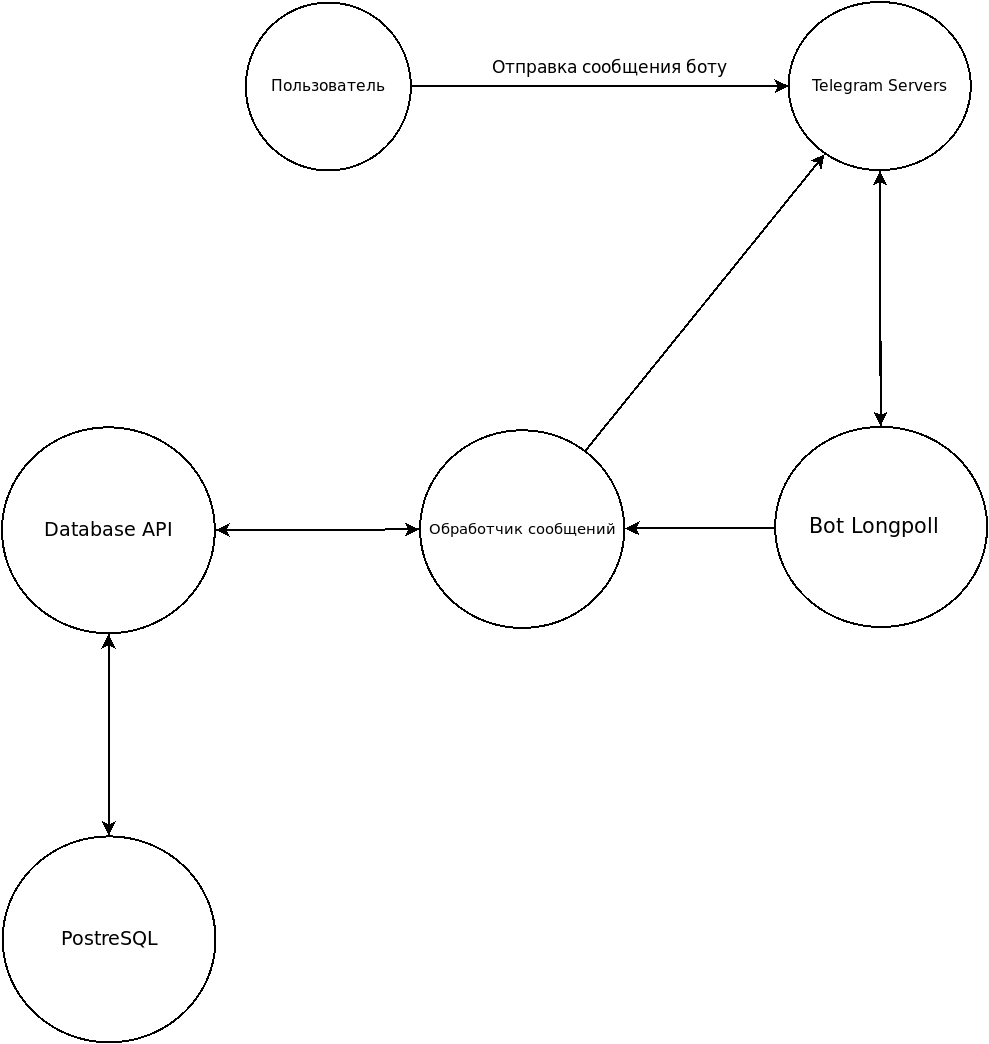
\includegraphics[scale=0.4]{High_level.png}
\end{figure}

\begin{figure}[!htb]
    \caption{Низкоуровневая диаграмма}
    \centering
    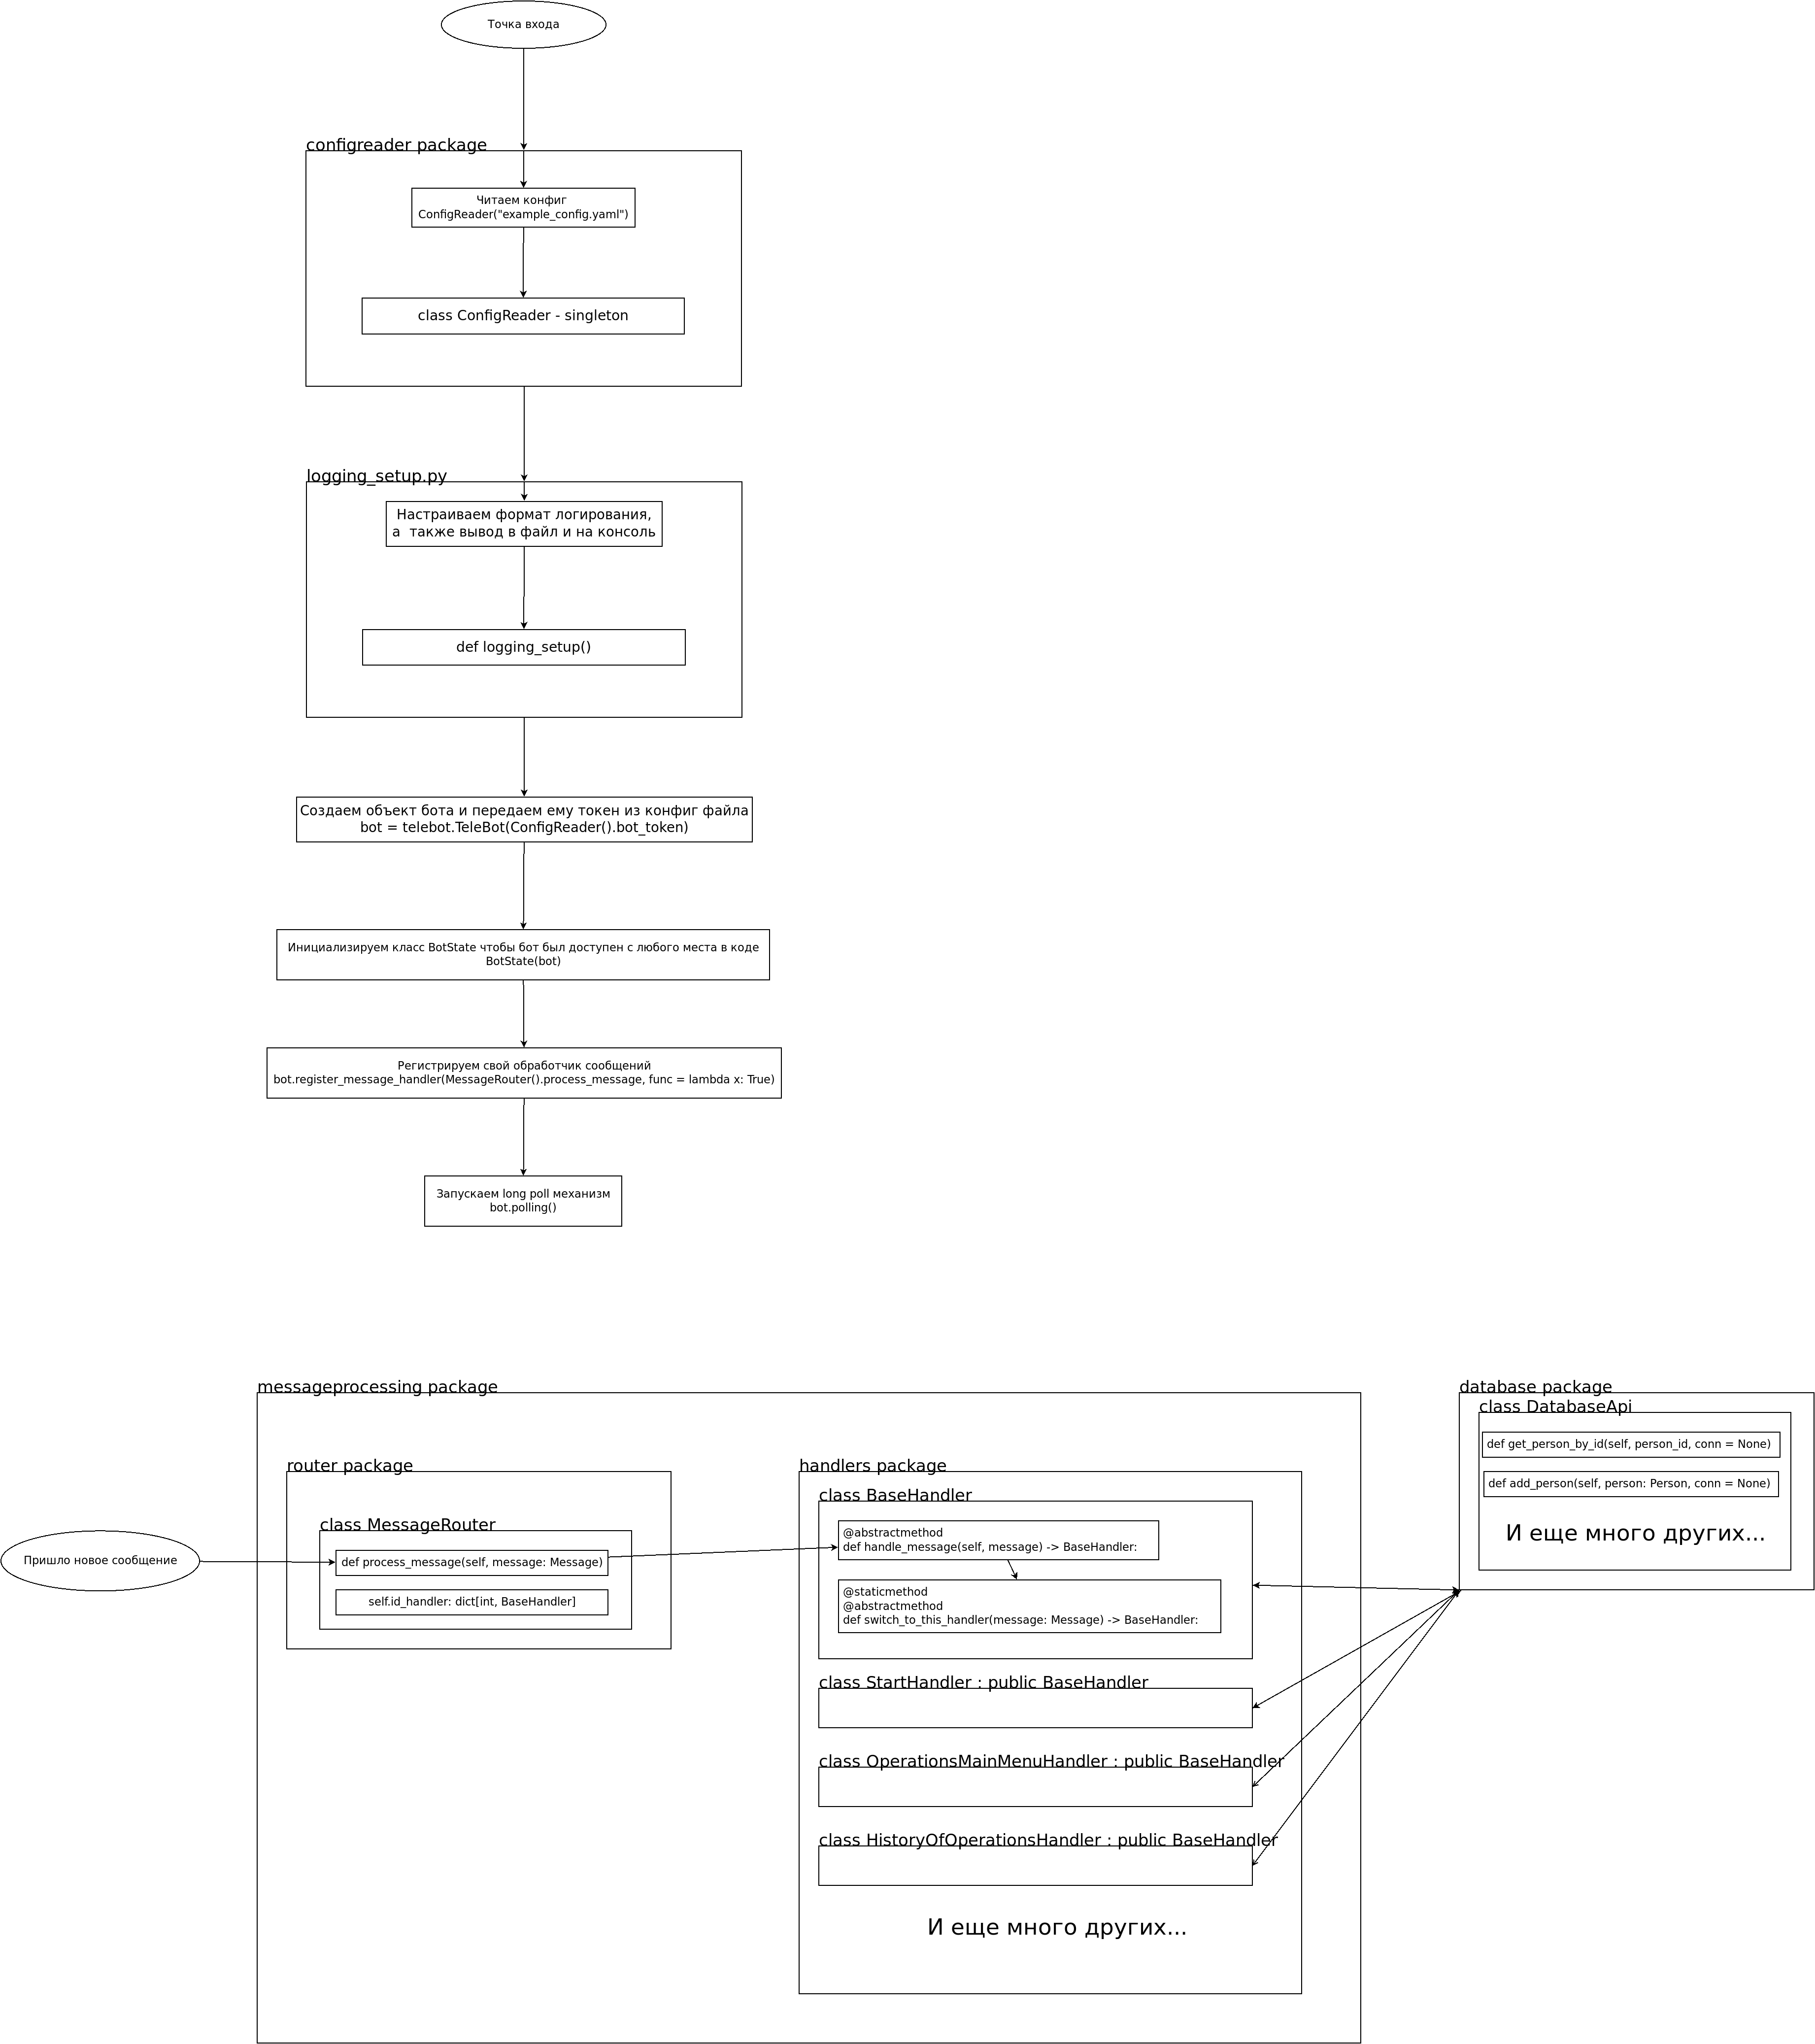
\includegraphics[scale=0.1]{Code_level.png}
\end{figure}

\pagebreak

\section{Заключение}
Мы научились красиво работать в команде над совместным проектом. Освоили новые методы проектирования, разработку на пайтоне, освоили создание контейнеров с базами данных в Docker Compose. Освоили совместную работу в Github.

\end{document}
